% !TEX encoding = UTF-8
% !TEX TS-program = pdflatex
% !TEX root = ../tesi.tex

%**************************************************************
\chapter{Progettazione e codifica}
\label{cap:progettazione-codifica}
%**************************************************************

\intro{In questo capitolo viene esposta la progettazione tecnica e la successiva codifica del prodotto ENTicketEngine.}\\
\section{Riferimenti}
    Di seguito vengono riportati i riferimenti ai vari tool e tecnologie previste per lo sviluppo del progetto:
    \begin{itemize}
        \item Java: \url{https://docs.oracle.com/en/java/javase/15/docs/api/index.html}
        \item API Redmine: \url{https://www.redmine.org/projects/redmine/wiki/rest_api}
        \item SDK Redmine: \url{https://github.com/taskadapter/redmine-java-api}
        \item Bot API Telegram: \url{https://core.telegram.org/bots}
        \item SDK Bot Telegram: \url{https://github.com/rubenlagus/TelegramBots}
        \item SDK Spring Mail: \url{https://mvnrepository.com/artifact/org.springframework.boot/spring-boot-starter-mail}
    \end{itemize}

\section{Analisi del prodotto}
	\subsection{Descrizione del prodotto}
		\subsubsection{Contesto}
			Il prodotto sarà utilizzato internamente dall'azienda Euronovate per il monitoraggio della validità delle \gloxy{S.L.A.}, e per un'analisi statistica delle segnalazioni aperte da \gloxy{Customers}.
			\subsubsection{Funzionalità}
			Il prodotto dovrà interfacciarsi con il software \gloxy{Redmine}, già utilizzato dall'azienda per la raccolta delle segnalazioni da parte dei clienti, per l'ottenimento dei dati, i quali poi dovranno essere analizzati e in caso di violazioni, saranno predisposti diversi canali di notifica, per la segnalazione della violazione.\\
			Infine, i dati saranno salvati in una base di dati, ed esposti tramite un \gloxy{API} con un fine di analisi statistica di essi.
			\newpage

\section{Analisi dell'architettura}
In questa sezione verrà analizzata l'architettura dei vari sistemi richiesti per la realizzazione del progetto\textbf{ENTicketEngine}.\\

    \subsection{Architettura}
        L'architettura del prodotto può essere riassunta con il seguente diagramma:
        \begin{center}
            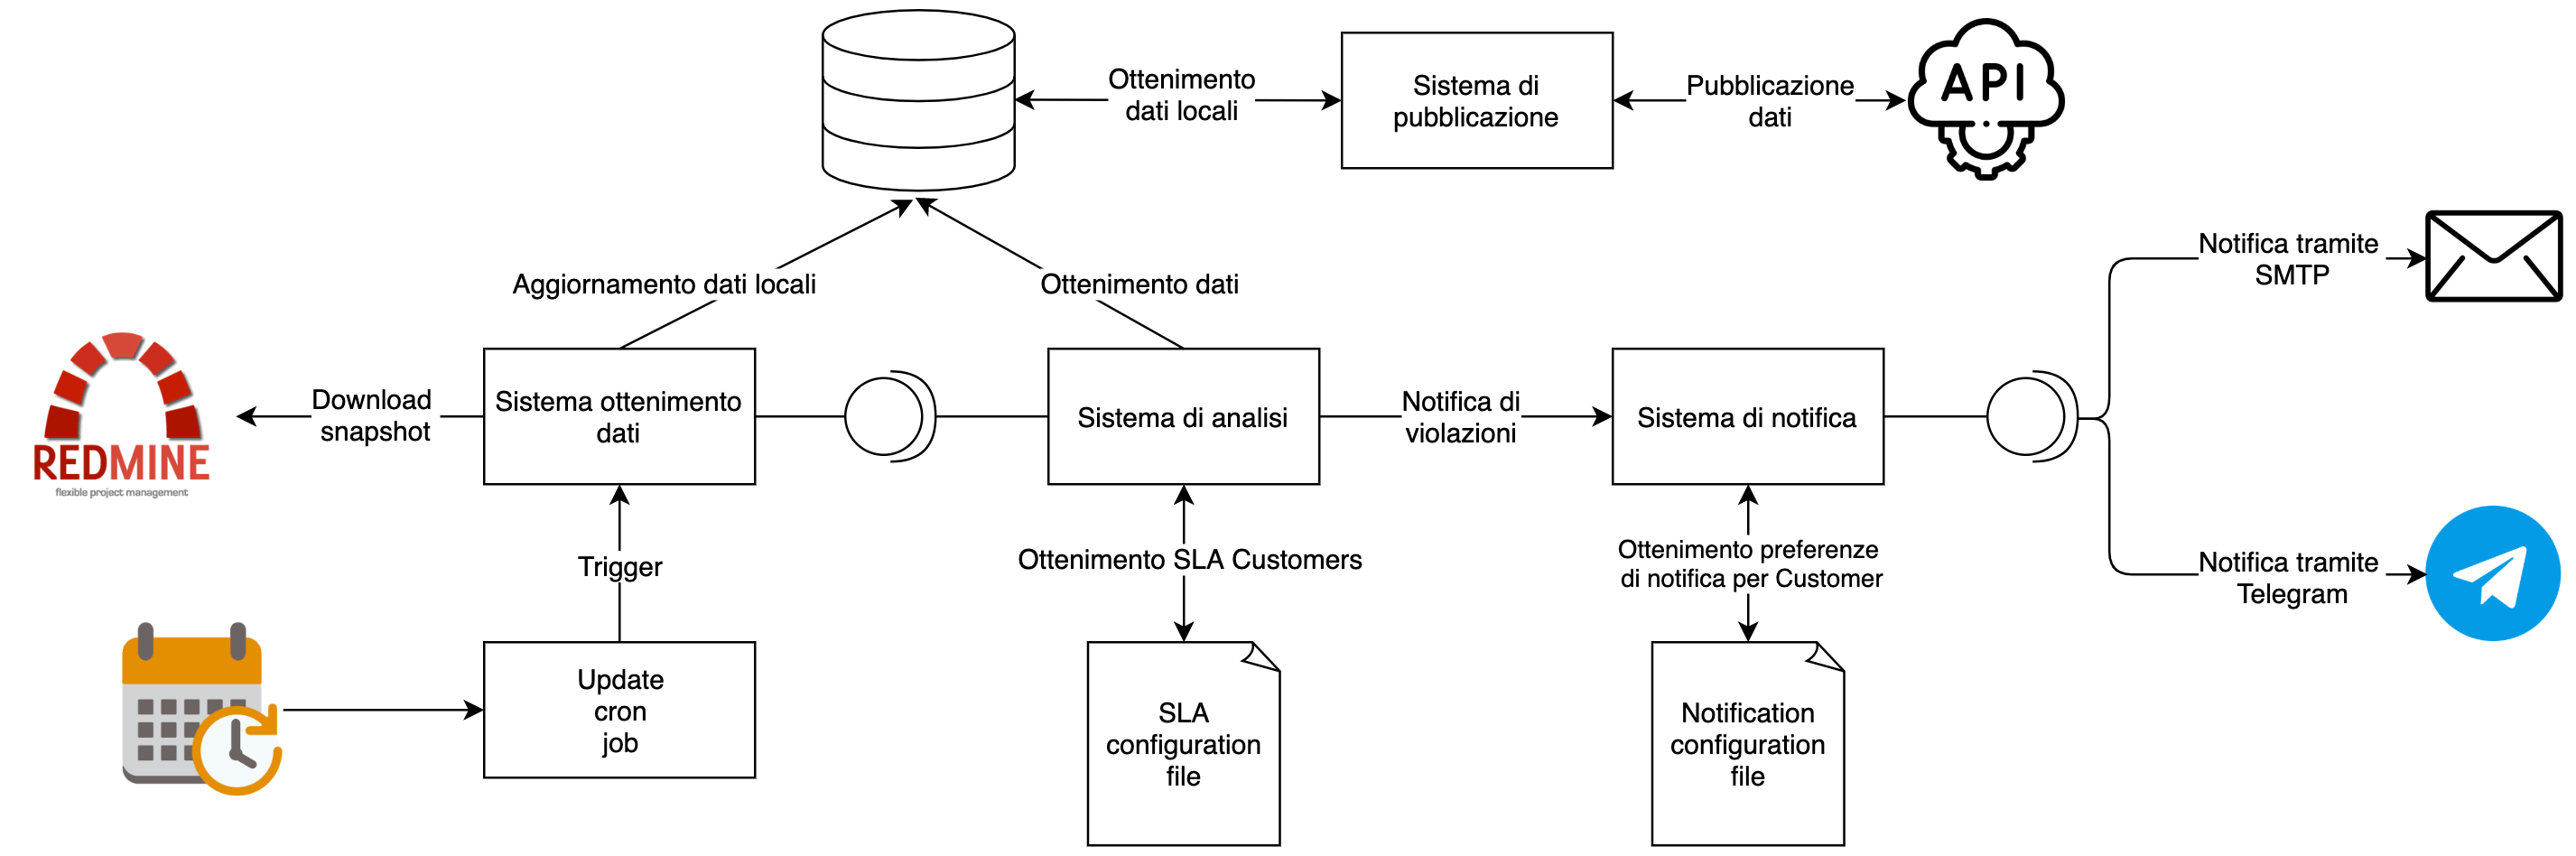
\includegraphics[keepaspectratio = true, width=15cm]{immagini/progettazione/architettura.png}
            \captionof{figure}{Architettura generale del prodotto}
        \end{center}
        \subsection{Analisi dei sistemi}
            Il prodotto prevede principalmente 4 sistemi: l'\gloxy{API} di pubblicazione, il sistema di ottenimento dei dati, il sistema di analisi, ed infine il sistema di notifica.
        \subsubsection{Sistema ottenimento dati}
            Questo sistema è responsabile dell'ottenimento dei dati da \gloxy{Redmine}, quali \gloxy{Customers} e \gloxy{Ticket} aperti da clienti. \\
            Tale quindi doveva autenticarsi su \gloxy{Redmine}, ottenere i dati, e manipolarli in modo da prevedere una loro semplice integrazione con gli altri servizi.
            Tale download dei dati è stato effettuato in batch, quindi periodicamente l'engine è andato a scaricarsi gli aggiornamenti. \\
             Infine, bisognava predisporre questo sistema in modo da permettere di migrare a un servizio di segnalazione esterno diverso da \gloxy{Redmine}, senza andare a modificare gli altri sistemi.
            \begin{quote}
            	\mbox{}%
            	\vspace{-1cm}
                \paragraph{Dettaglio tecnico}
	                \mbox{}\\
                    Questo sistema essendo responsabile dell'ottenimento dei dati, si è dovuto appoggiare al servizio esterno scelto (in questo caso, \gloxy{Redmine}) per il raggiungimento del suo scopo. \\
                    Da Analisi dei Requisiti risulta un requisito che tale sistema però possa in futuro essere cambiato facilmente: ciò implica che il sistema di ottenimento dati debba essere il più possibile disaccoppiato dal sistema con il quale si andrà a interfacciare. \\
                    Per far ciò quindi, si è proceduto a creare un modulo per interfacciarsi al servizio esterno, che è stato accoppiato al sistema di ottenimento dati tramite \texttt{(Object) Adapter design pattern}.
                    \subparagraph*{Dipendenze esterne}
                    \mbox{} \\
                        Questo sistema si può scomporre in 2 sottosistemi:
                        \begin{enumerate}
                            \item un sottosistema per ottenere i dati;
                            \item un sottosistema per salvare gli oggetti ottenuti nella base di dati.
                        \end{enumerate}
                        Il tutto è rappresentato nel seguente grafico:
                        \begin{center}
                            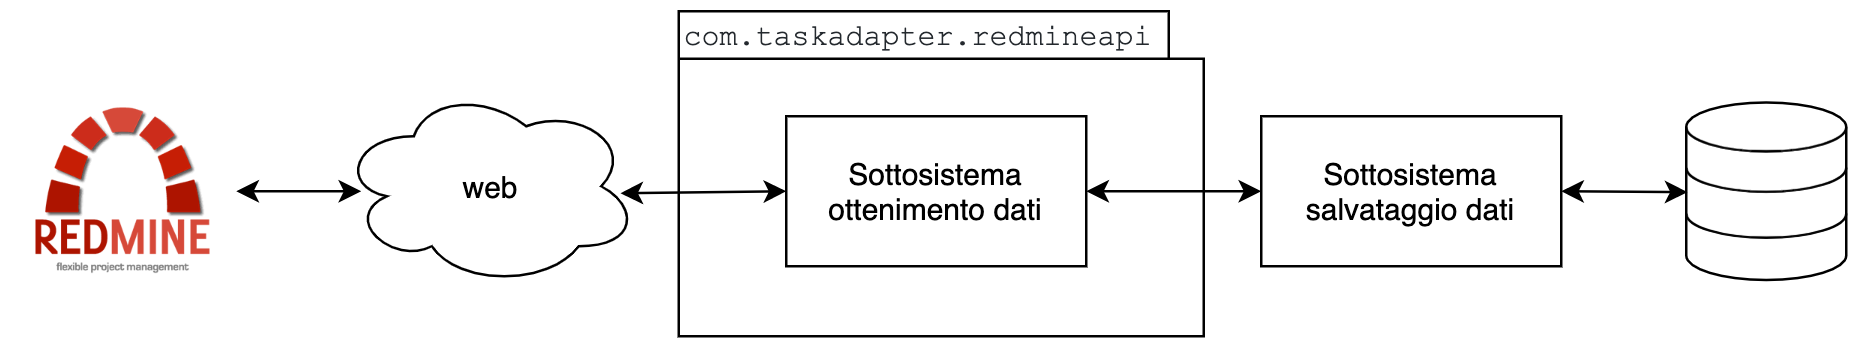
\includegraphics[keepaspectratio = true, width=14cm]{immagini/progettazione/ottenimento.png}
                            \captionof{figure}{Struttura del sistema di ottenimento}
                        \end{center}
                        Come si può notare dal diagramma, fa uso della dipendenza \texttt{com.taskadapter:redmine-java-api} per andare a interfacciarsi con Redmine.
            \end{quote}
        \subsubsection{Sistema analisi dati}
            Questo sistema è responsabile dell'analisi dei dati e delle \gloxy{S.L.A.}. definite con i vari clienti. \\
            È stato quindi necessario predisporre un sistema di configurazione delle \gloxy{S.L.A.}. dei clienti dinamico, che non richiedesse il riavvio del sistema. \\
            Una volta analizzato dati e \gloxy{S.L.A.}., è responsabile  della comunicazione con il servizio di notifica per la segnalazione di violazioni.
            \begin{quote}
            	\mbox{}%
            	\vspace{-1cm}
                \paragraph{Dettaglio tecnico}
                	 \mbox{}\\
                    Questo sistema essendo responsabile della notifica delle violazioni, doveva prevedere degli algoritmi, che date le configurazioni lette inizialmente, analizzeranno i dati per trovare violazioni o segnalazioni. \\
                    Considerato che le necessità e i vincoli potevano cambiare, è stato usato \texttt{Strategy design pattern} per l'algoritmo, e considerato che le configurazioni delle \gloxy{S.L.A.} sono componibili (possono avere o meno una durata massima di presa in carico, possono o meno avere una durata massima di risoluzione, ecc ecc), si poteva far uso di \texttt{Decorator design pattern} per la logo generazione da file.
                    \subparagraph{Dipendenze esterne}
                    \mbox{} \\
                        Non sono state identificate dipendenze esterne per questo sistema.
            \end{quote}
        \subsubsection{Sistema di notifica}
            Questo sistema è responsabile della notifica delle violazioni ai responsabili.\\
            È stato quindi necessario predisporre vari mezzi di notifica, configurabili dinamicamente, che permettano la segnalazione a chi di dovere della potenziale violazione delle \gloxy{S.L.A.}., in base a quanto grave essa sia.
            \begin{quote}
            	\mbox{}%
            	\vspace{-1cm}
                \paragraph{Dettaglio tecnico}
                	 \mbox{}\\
                    Questo sistema, per raggiungere il suo obiettivo, doveva interfacciarsi con sistemi esterni, per i quali esistono già \gloxy{SDK} completi e testati. \\
                    Per permettere la modularità di tale sistema, e la possibilità di integrare nuovi canali di notifica senza andare a modificare codice pre-esistente, si è fatto uso del \texttt{Adapter design pattern} per conformare tutti i canali sotto un unica interfaccia, e nel caso tali SDK non fossero esistiti, si avrebbe fatto uso dell'\texttt{ereditarietà} per la loro creazione.
                    \subparagraph{Dipendenze esterne}
                    \mbox{} \\
                        Questo sistema si può scomporre in 2 sottosistemi:
                        \begin{enumerate}
                            \item un sottosistema per la gestione dei canali di notifica;
                            \item un sottosistema per ogni canale di notifica.
                        \end{enumerate}
                        Il tutto è rappresentato nel seguente grafico:
                        \begin{center}
                            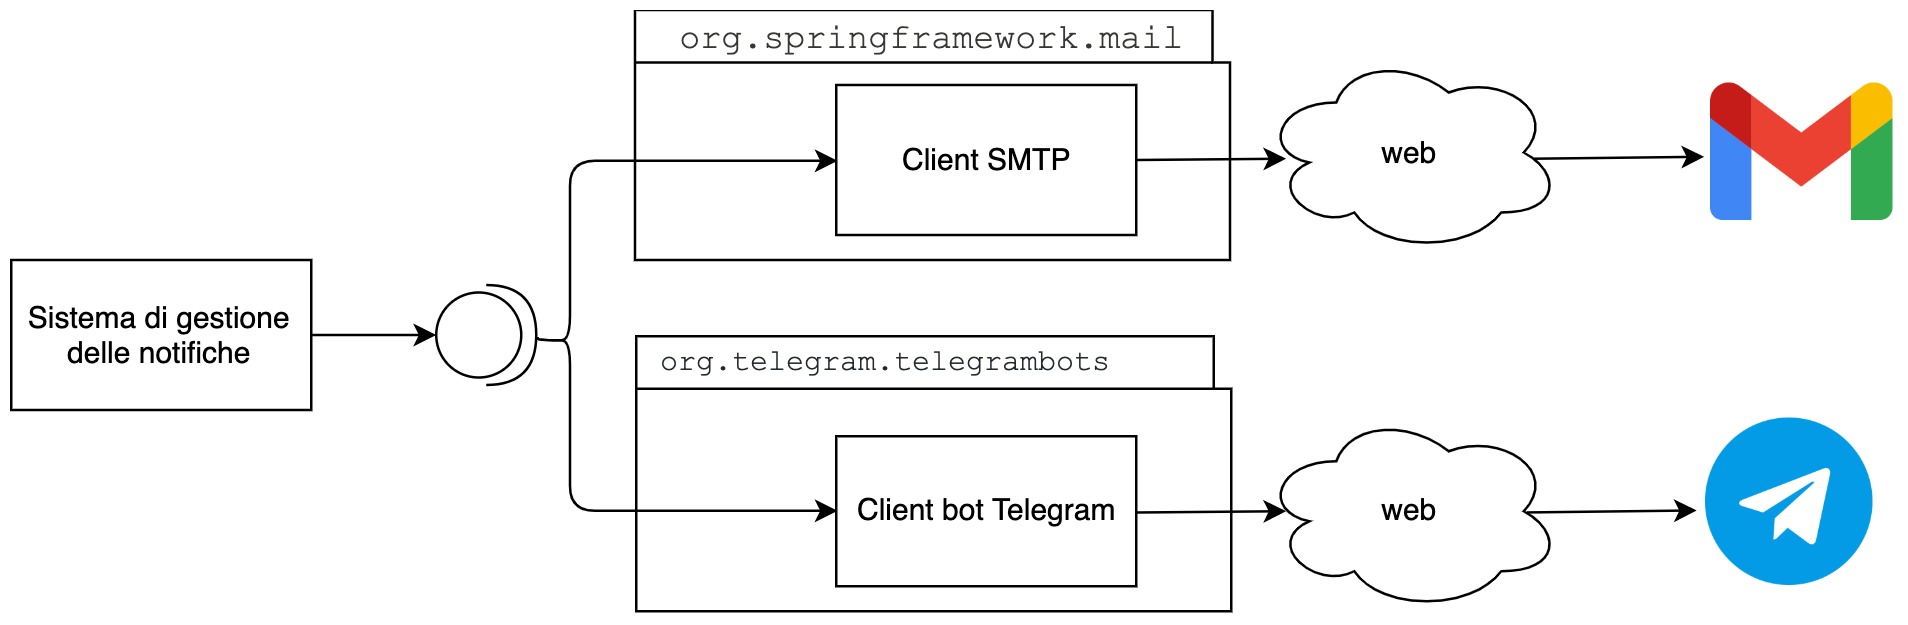
\includegraphics[keepaspectratio = true, width=14cm]{immagini/progettazione/notifica.png}
                            \captionof{figure}{Struttura del sistema di notifica}
                        \end{center}
                        Come si può notare dal diagramma, fa uso delle seguenti dipendenze:
                        \begin{itemize}
                            \item \texttt{org.springframework.boot:spring-boot-starter-mail} per andare a interfacciarsi con Gmail per la notifica tramite mail;
                            \item \texttt{org.telegram:telegrambots} per andare a interfacciarsi con Telegram per la notifica tramite messaggio su gruppo.
                        \end{itemize} 
            \end{quote}
        \subsubsection{Sistema di pubblicazione}
            Questo sistema è responsabile della pubblicazione dei dati gestiti verso l'esterno.\\
            È stato quindi necessario predisporre un \gloxy{API} tramite la quale gli interessati potranno accedere alle informazioni gestite dall'engine, quali issue, customer e violazioni. \\
            \begin{quote}
            	\mbox{}%
            	\vspace{-1cm}
                \paragraph{Dettaglio tecnico}
                	 \mbox{}\\
                    Questo sistema, avente come responsabilità la pubblicazione di analisi statistiche sui dati, ha fatto uso del \texttt{MVC design pattern} per il suo sviluppo, così da disaccoppiare la logica tra modello, controller e viste, in modo da rendere modulare il sistema e permettere una potenziale futura migrazione a tipi di viste diverse (per esempio tramite XML) o l'aggiunta di nuovi endpoint.\\
                    \subparagraph{Dipendenze esterne}
                    \mbox{} \\
                        Questo sistema è stato, come precedentemente dichiarato, sviluppato seguendo il design pattern MVC, questo appoggiandosi al framework Java, Spring Boot. \\
                        Per questo motivo viene identificato \texttt{org.springframework.boot} come dipendenza esterna. 
            \end{quote}
        \newpage
    \subsection{Logica dell'engine}
        La logica che usa l'engine per raggiungere i suoi obbiettivi può essere riassunta con il seguente diagramma UML:
                \begin{center}
            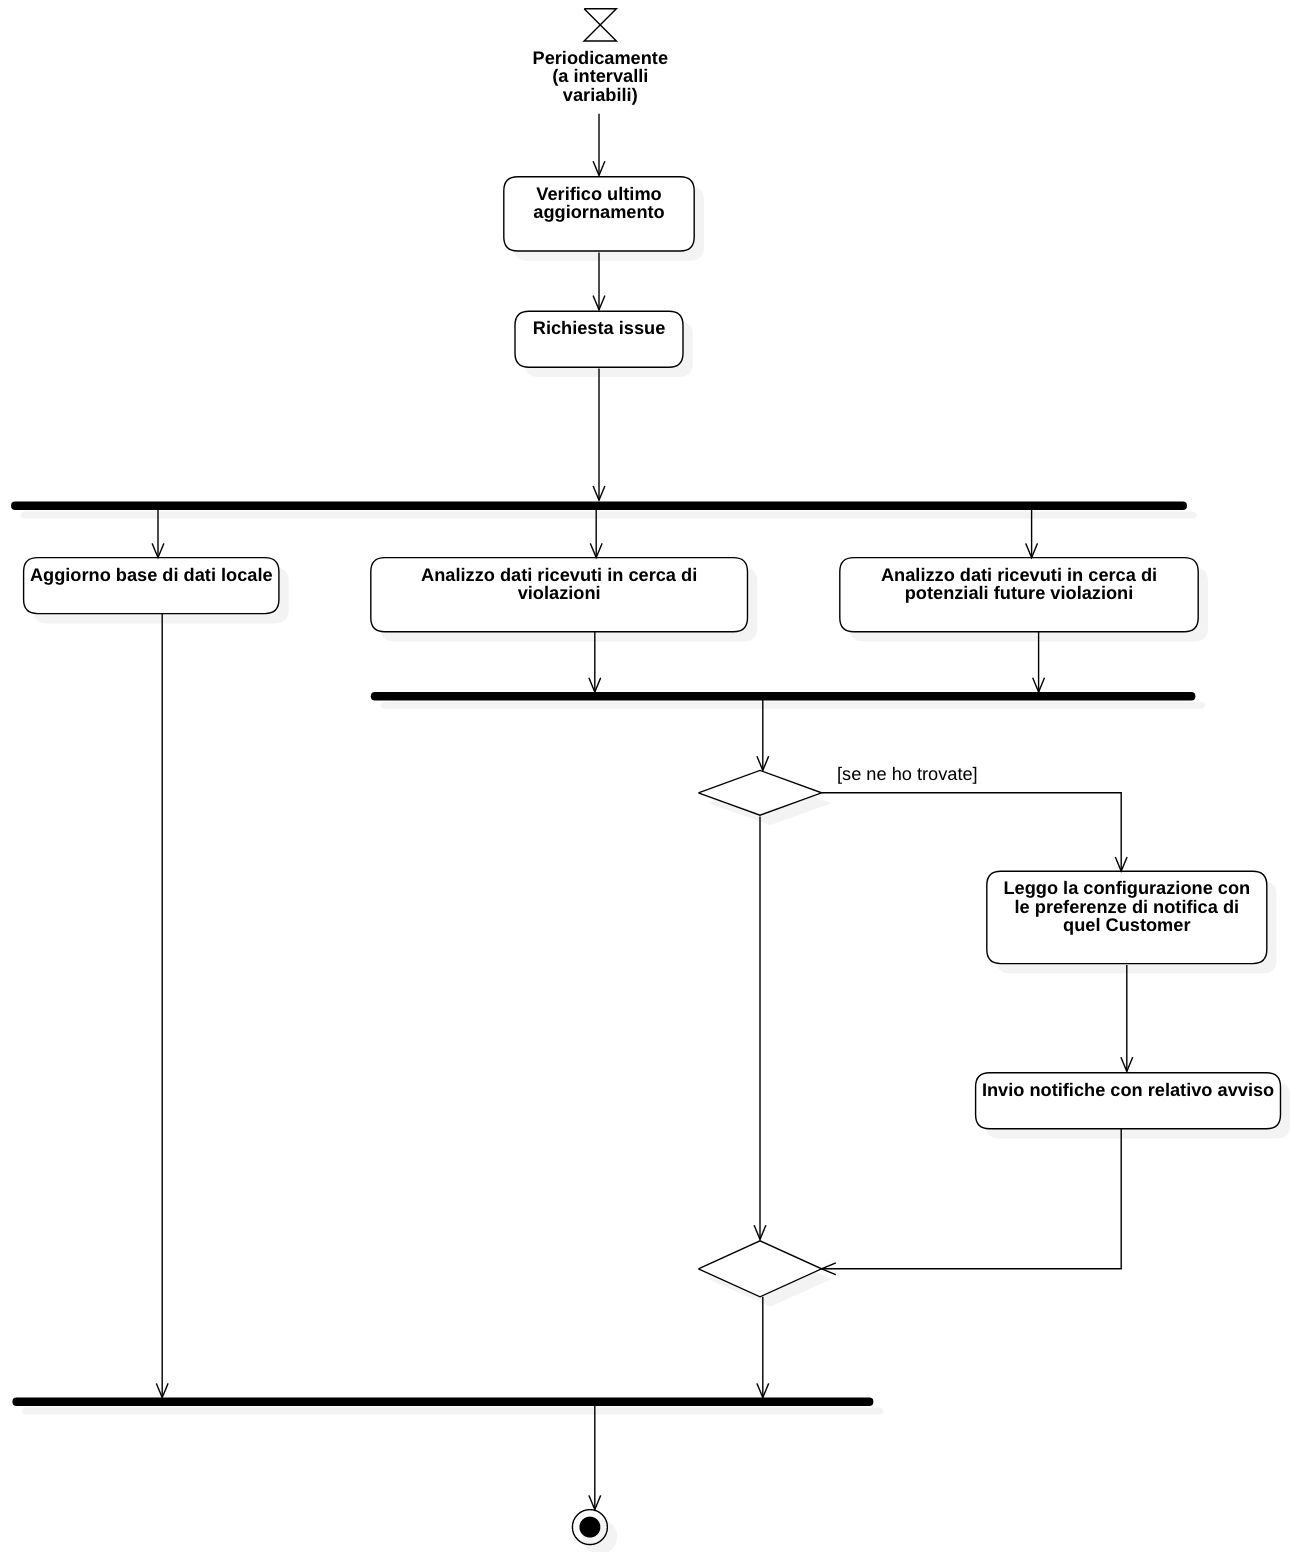
\includegraphics[keepaspectratio = true, width=16.5cm]{immagini/progettazione/activity.png}
            \captionof{figure}{Diagramma di attività dell'algoritmo dell'engine}
        \end{center}
    
        
\section{Base di dati}
    Il progetto prevede l'uso di una base di dati per il mantenimento locale delle informazioni ottenute dal servizio esterno per la gestione di progetto. \\
    In particolare, questa base di dati ha l'obiettivo di mantenere le informazioni esposte dall'API successivamente descritta. \\
    \par La base di dati prevista è rappresentata dal seguente schema ER:
    \begin{center}
        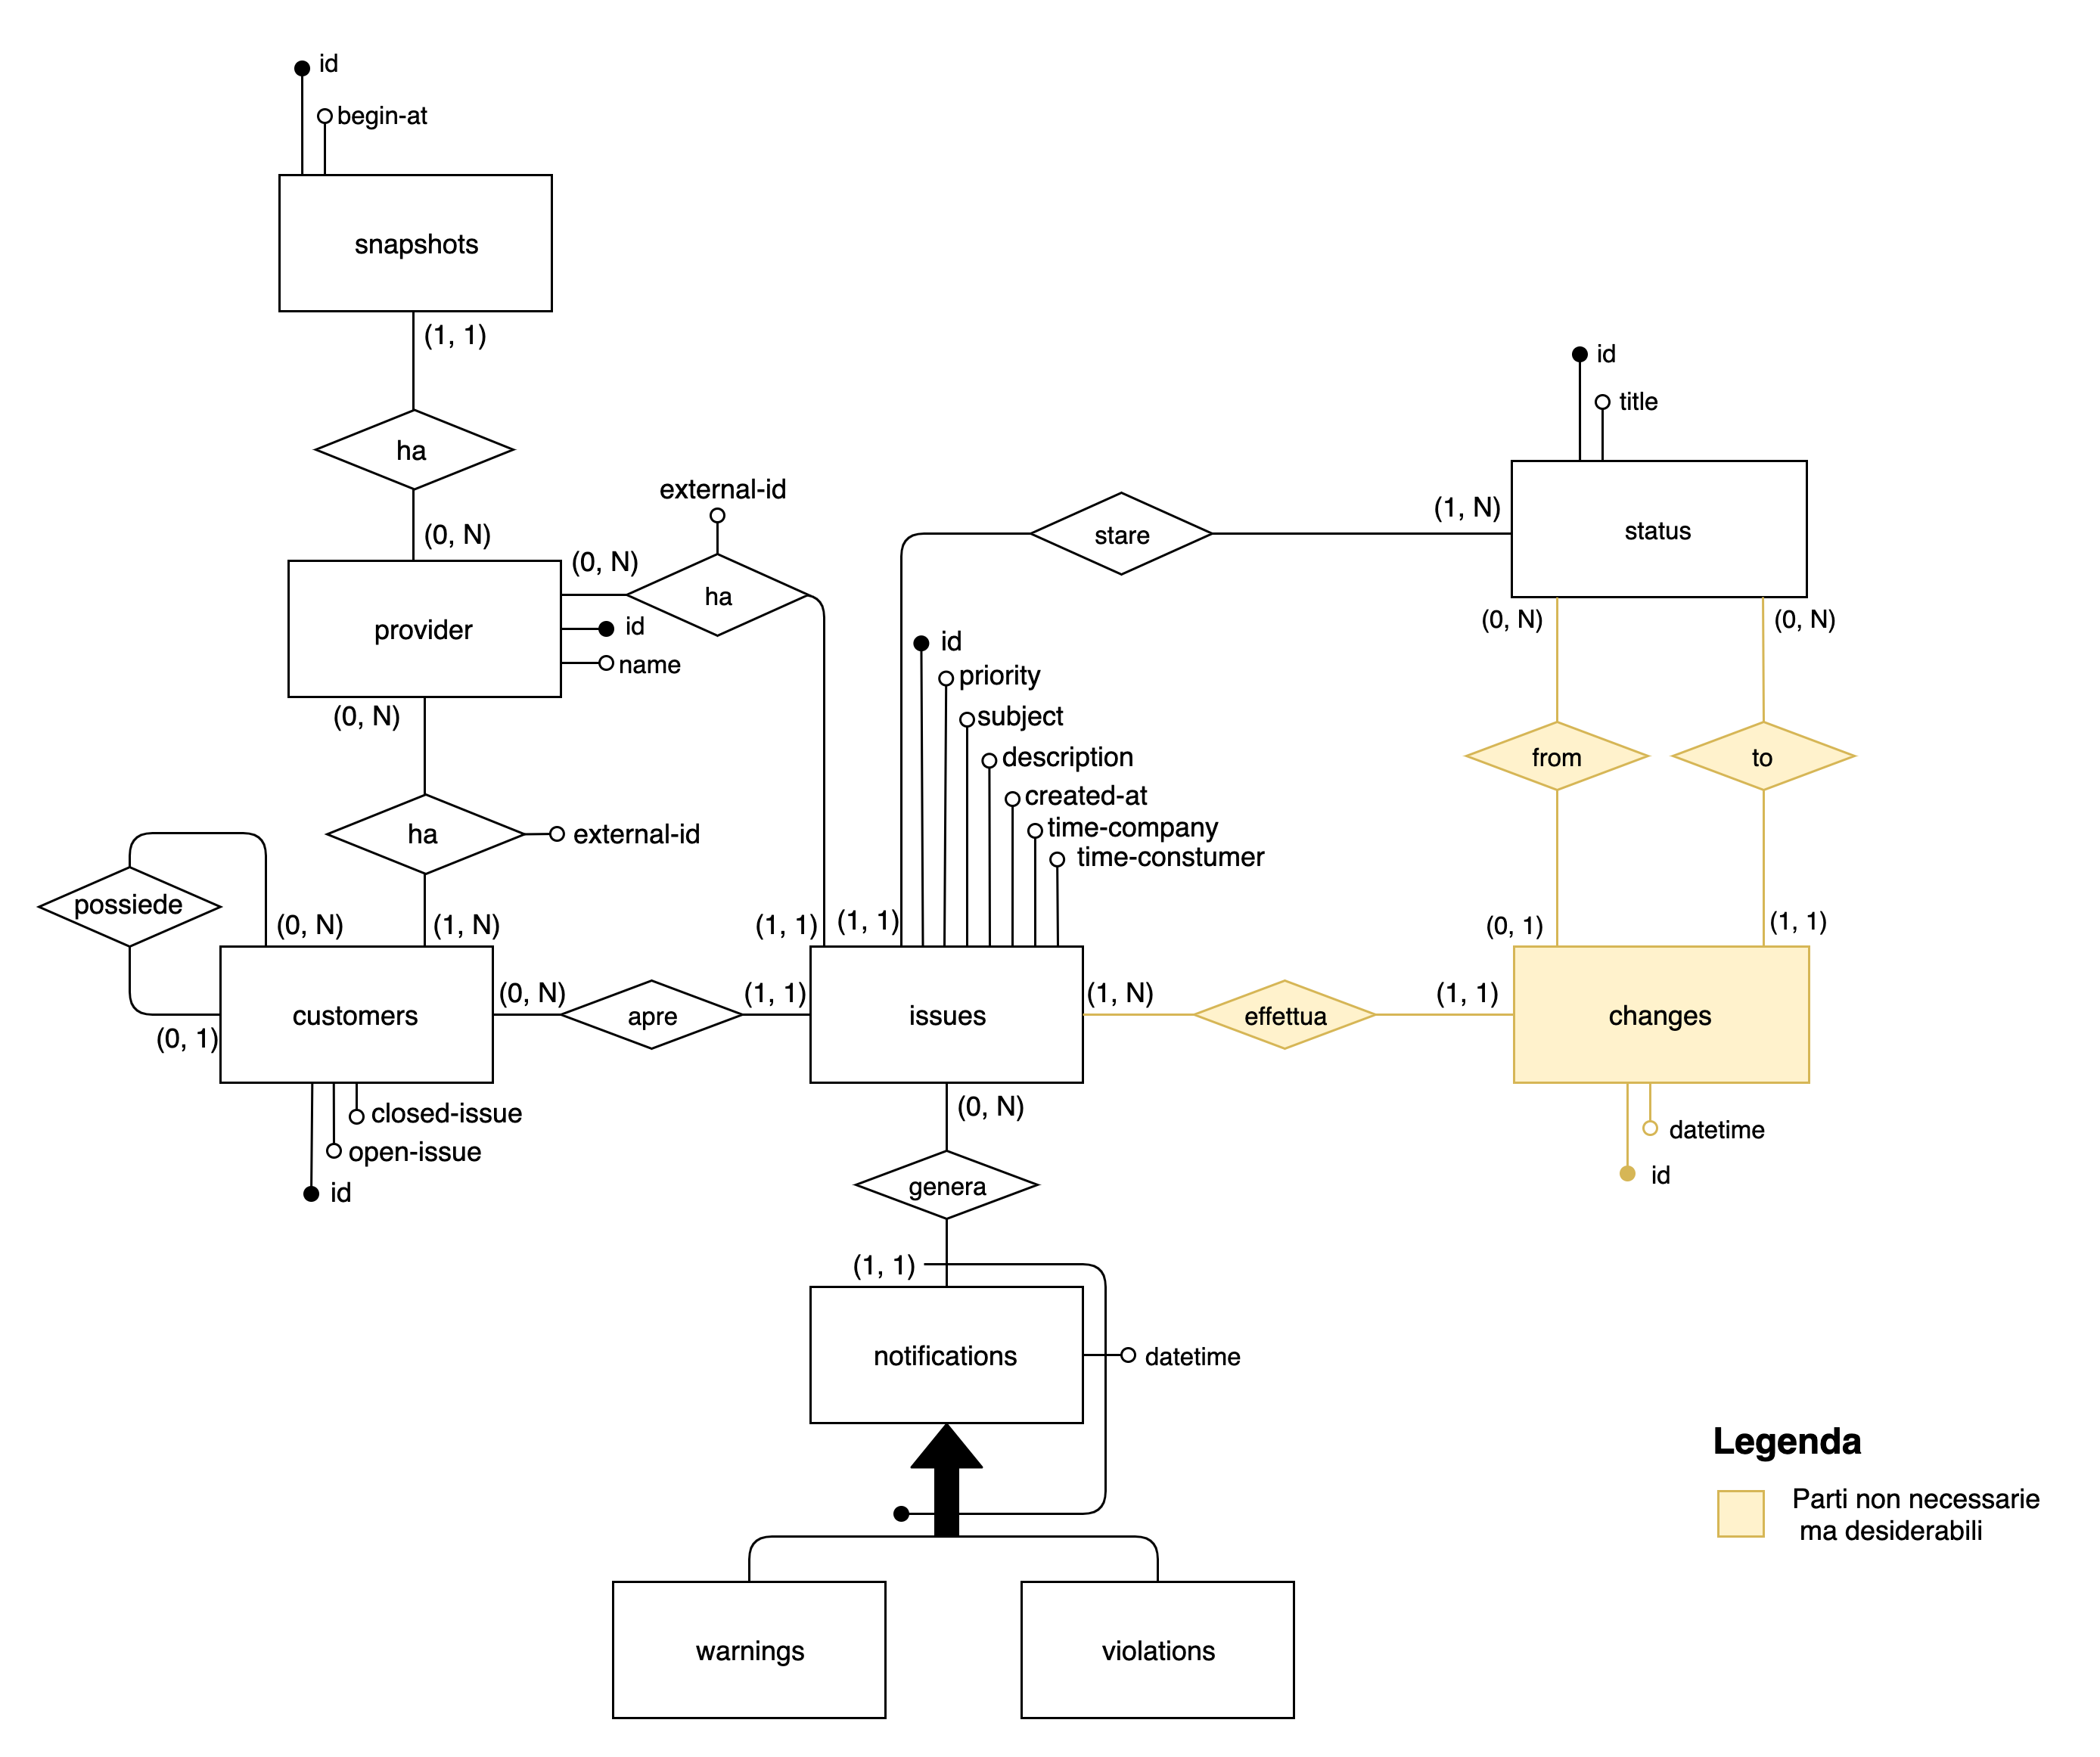
\includegraphics[keepaspectratio = true, width=15cm]{immagini/progettazione/db.png}
        \captionof{figure}{Struttura della base di dati prevista}
    \end{center}
    \subsection{Analisi ridondanze}
        Lo schema ER visibile alla sezione precedente, presenta non minimalità, quali:
        \begin{itemize}
            \item \texttt{status} in \texttt{issues}, che potrebbe essere recuperato dallo stato del suo ultimo cambiamento;
            \item \texttt{time-company} e \texttt{time-customer} in \texttt{issues} che potrebbero essere ricalcolate considerando tutti le sue \texttt{changes};
            \item \texttt{open-issue} e \texttt{closed-issue} in \texttt{customers} che potrebbero essere ottenute contando le \texttt{issues} associate.
        \end{itemize} 
        Si è deciso di mantenere queste non-minimalità in modo da ottimizzare la pubblicazione di suddetti dati dall'API, in quanto focus primario del progetto.
    








\section{Endpoint API}
    \subsection{/customer/\{customer-id\}}
        \begin{itemize}
            \item \textbf{Tipo del metodo}: GET;
            \item \textbf{Descrizione}: endpoint per l'ottenimento delle informazioni rispetto a un customer.
            \item \textbf{Parametri}: \\
            \begin{center}
                \rowcolors{2}{lightest-grayest}{white}
                \begin{longtable}{|p{4cm}|p{4cm}|p{6cm}|}
                    \hline
                    \rowcolor{lighter-grayer}
                    \textbf{Nome} & \textbf{Tipo} & \textbf{Descrizione} \\ \hline
                    \texttt{min} & Timestamp GMT+2 & Data minima dell'apertura di ticket da considerare \\ \hline
                    \texttt{max} & Timestamp GMT+2 & Data massima dell'apertura di ticket da considerare \\ \hline
                \end{longtable}
            \end{center}
            \item \textbf{Risposte}: 
            \begin{center}
                \rowcolors{2}{lightest-grayest}{white}
                \begin{longtable}{|p{2.5cm}|p{5.5cm}|p{6cm}|}
                    \hline
                    \rowcolor{lighter-grayer}
                    \textbf{Identificativo} & \textbf{Schema \gloxy{JSON}} & \textbf{Descrizione} \\
                    \hline
                    \endfirsthead
                    200 & 
                    \texttt{
                        \{ \newline 
                            "id": int \newline 
                            "name": string \newline 
                            "issues": int \newline 
                            "violations": int \newline 
                            "avg-pending": float \newline 
                            "avg-resolved": float \newline 
                        \}
                    } 
                    & Risposta contenente:
                    \begin{itemize}
                        \item nome del customer
                        \item numero di issue aperte
                        \item numero di violazioni subite
                        \item tempo medio di presa in carico
                        \item tempo medio di risoluzione
                    \end{itemize}
                    \\ \hline
                    400 & \texttt{\{ \newline "message": string \newline \}} & I timestamp forniti non sono validi
                    \\ \hline
                    404 & \texttt{\{ \newline "message": string \newline \}} & L'id del customer fornito non è stato trovato
                    \\ \hline
                \end{longtable}
            \end{center}
            \item \textbf{HTTP headers}: 
            \begin{itemize}
                \item \textbf{Content-Type:} \texttt{application/json} ;
            \end{itemize}
        \end{itemize}
    
    
    \newpage
    \subsection{/issue/\{issue-id\}}
        \begin{itemize}
            \item \textbf{Tipo del metodo}: GET;
            \item \textbf{Descrizione}: endpoint per l'ottenimento delle informazioni rispetto a un issue.
            \item \textbf{Parametri}: \\
            Nessuno
            \item \textbf{Risposte}: 
            \begin{center}
                \rowcolors{2}{lightest-grayest}{white}
                \begin{longtable}{|p{2.5cm}|p{5.5cm}|p{6cm}|}
                    \hline
                    \rowcolor{lighter-grayer}
                    \textbf{Identificativo} & \textbf{Schema \gloxy{JSON}} & \textbf{Descrizione} \\
                    \hline
                    \endfirsthead
                    200 & 
                    \texttt{
                        \{ \newline 
                        "id": int \newline 
                        "customer": int \newline 
                        "status": string \newline 
                        "priority": string \newline 
                        "subject": string \newline 
                        "description": string \newline 
                        "start-date": string(yyyy-mm-gg) \newline 
                        "time-company": int \newline 
                        "time-client": int \newline 
                        \}
                    } 
                    & Risposta contenente :
                    \begin{itemize}
                        \item id dell'issue
                        \item nome del customer
                        \item stato dell'issue
                        \item priorità dell'issue
                        \item oggetto dell'issue
                        \item descrizione dell'issue
                        \item data di apertura dell'issue
                        \item tempo che è stato in carico a Euronovate
                        \item tempo che è stato in carico al Customer
                    \end{itemize}
                    \\ \hline
                    404 & \texttt{\{ \newline "message": string \newline \}} & L'id dell'issue fornito non è stato trovato
                    \\ \hline
                \end{longtable}
            \end{center}
            \item \textbf{HTTP headers}: 
            \begin{itemize}
                \item \textbf{Content-Type:} \texttt{application/json} ;
            \end{itemize}
        \end{itemize}
    
    
    
    
    \newpage
    \subsection{/issues}
        \begin{itemize}
            \item \textbf{Tipo del metodo}: GET;
            \item \textbf{Descrizione}: endpoint per ottenere informazioni statistiche sull'andamento nel tempo delle issue.
            \item \textbf{Parametri}: \\
                \begin{center}
                    \rowcolors{2}{lightest-grayest}{white}
                    \begin{longtable}{|p{4cm}|p{4cm}|p{6cm}|}
                        \hline
                        \rowcolor{lighter-grayer}
                        \textbf{Nome} & \textbf{Tipo} & \textbf{Descrizione} \\ \hline
                        \texttt{min} & Timestamp GMT+2 & Data minima dell'apertura di ticket da considerare \\ \hline
                        \texttt{max} & Timestamp GMT+2 & Data massima dell'apertura di ticket da considerare \\ \hline
                        \texttt{group-by} & string & String rappresentante la politica di raggruppamento; deve essere una tra:
                        \begin{itemize}
                            \item day
                            \item month (default)
                            \item year
                        \end{itemize}
                            \\ \hline
                    \end{longtable}
                \end{center}
            \item \textbf{Risposte}: 
            \begin{center}
                \rowcolors{2}{lightest-grayest}{white}
                \begin{longtable}{|p{2.5cm}|p{5.5cm}|p{6cm}|}
                    \hline
                    \rowcolor{lighter-grayer}
                    \textbf{Identificativo} & \textbf{Schema \gloxy{JSON}} & \textbf{Descrizione} \\
                    \hline
                    \endfirsthead
                    200 & 
                    \texttt{
                        [
                        \{ \newline 
                        "begin-date": string (yyyy-mm-gg) \newline 
                        "created-issues": int \newline 
                        "open-issues": int \newline 
                        "violations": int \newline 
                        \},\newline 
                        ...\newline 
                        ]
                    } 
                    & Risposta contenente una collezione di oggetti contenenti:
                    \begin{itemize}
                        \item la data di inizio periodo
                        \item numero di issue aperte in quel periodo
                        \item numero di issue aperte all'inizio di quel periodo 
                        \item numero di violazioni notificate in quel periodo
                    \end{itemize}
                    \\ \hline
                    400 & \texttt{\{ \newline "message": string \newline \}} & I timestamp forniti non sono validi o il campo di raggruppamento non contiene uno dei valori definiti.
                    \\ \hline
                \end{longtable}
            \end{center}
            \item \textbf{HTTP headers}: 
            \begin{itemize}
                \item \textbf{Content-Type:} \texttt{application/json} ;
            \end{itemize}
        \end{itemize}
    \newpage
    
    
    
    
    
    
    
    
    
    
\section{Sviluppo}
	In questa sezione verranno trattate la parti principali e più interessanti della codifica e realizzazione del progetto.
	\subsection{Tecnologie e strumenti}
		Durante la fase di sviluppo son stati necessari strumenti per la verifica e lo sviluppo dei vari componenti, quali:
		\begin{itemize}
			\item Java : linguaggio con il quale si è sviluppato il progetto per la maggior parte, principalmente la sua versione 11 LTS
			\item JSON : markup usato per la pubblicazione dei dati dell'API
			\item XML : markup usato per il salvataggio dei dati sui customers, sui canali di notifica e sugli orari di lavoro su disco
			\item Git : sistema di versionamento usato per il tracciamento del progetto
			\item CodeCommit : servizio di hosting online per repository che supporta Git, di proprietà AWS
			\item Spring Boot : framework principale del progetto a base Java, estremamente diffuso in ambito aziendale/lavorativo
			\item Redmine SDK : libreria usata per interfacciarsi con le API di Redmine
			\item Telegram SDK : libreria usata per interfacciarsi con le API di Telegram
			\item Spring Mail : libreria usata per interfacciarsi con server mail
			\item IntelliJ IDEA : IDE usato per lo sviluppo del progetto
			\item JUnit : libreria Java per lo sviluppo di test di unità
			\item Postman : applicazione per interrogazione e testing di API
			\item Docker : prodotto usato per il deploy finale del prodotto
			\item SQL : linguaggio per database basati sul modello relazionale, usato per il mantenimento dei dati, in particolare usato con DMBS  PostgreSQL
			\item pgAdmin : client per la gestione di DBMS PostgreSQL
		\end{itemize}
	\subsection{Ordine di sviluppo}
		Come descritto in precedenza, il prodotto prevede dei sistemi isolati tra di loro, ognuno con il proprio obiettivo. \\
		Appunto per la loro peculiarità di essere isolati, si è proceduto allo sviluppo di ognuno di essi in modo sequenziale, passando al successivo solo quando quello corrente è completo e funzionante. \\
		In particolare, lo sviluppo ha seguito il seguente ordine:
		\begin{enumerate}
			\item Base di dati
			\item Layer di persistenza
			\item Sistema di ottenimento
			\item Sistema di aggiornamento
			\item Sistema di analisi
			\item Sistema di notifica
			\item Sistema di pubblicazione
		\end{enumerate}
		Successivo allo sviluppo di ognuno di questi punti, si è svolto un allineamento con il tutor aziendale, per assicurarsi che il sistema prodotto fosse completo e funzionale.\\
		Seguendo questo ordine è stato più facile sviluppare i sistemi il più isolati possibili, e quindi concentrandosi sugli obiettivi di essi e il come potessero essere usati, ma non come sarebbero stati usati. \\
	\subsection{Differenze dalla progettazione}
		Per quanto il prodotto sviluppato assomigli molto a quello pensato durante la fase di progettazione, son state necessarie alcune modifiche, per correggere alcuni aspetti non previsti in fasi precedenti, in particolare:
		\begin{itemize}
			\item Sistema di aggiornamento: questo sistema non era previsto dalla progettazione, ma considerata la tarda notifica della granularità dei vincoli presenti nelle SLA, è stato necessario introdurlo per mantenere consistenti le non minimalità presenti nella base di dati.
			\item Algoritmo calcolo tempo su orario lavorativo: è stato necessario lo sviluppo di alcune classi di supporto per i vari sistemi per la gestione delle tempistiche con ottica lavorativa, quindi considerando un orario lavorativo.
			\item Algoritmo di invio di notifiche estendibile per le varie necessità dei canali, per evitare di andare a violare definiti dai rate limiter dei vari sistemi esterni.
			\item sviluppo di un orchestratore per i vari manager dei vari sistemi (Engine)
		\end{itemize}
		Questi nuovi componenti non hanno però portato un ritardo allo sviluppo in quanto fondamentali ma relativamente semplici da implementare. \\
		Considerate queste modifiche, il progetto finale ha un architettura che può essere descritta dal seguente schema:
		\begin{center}
			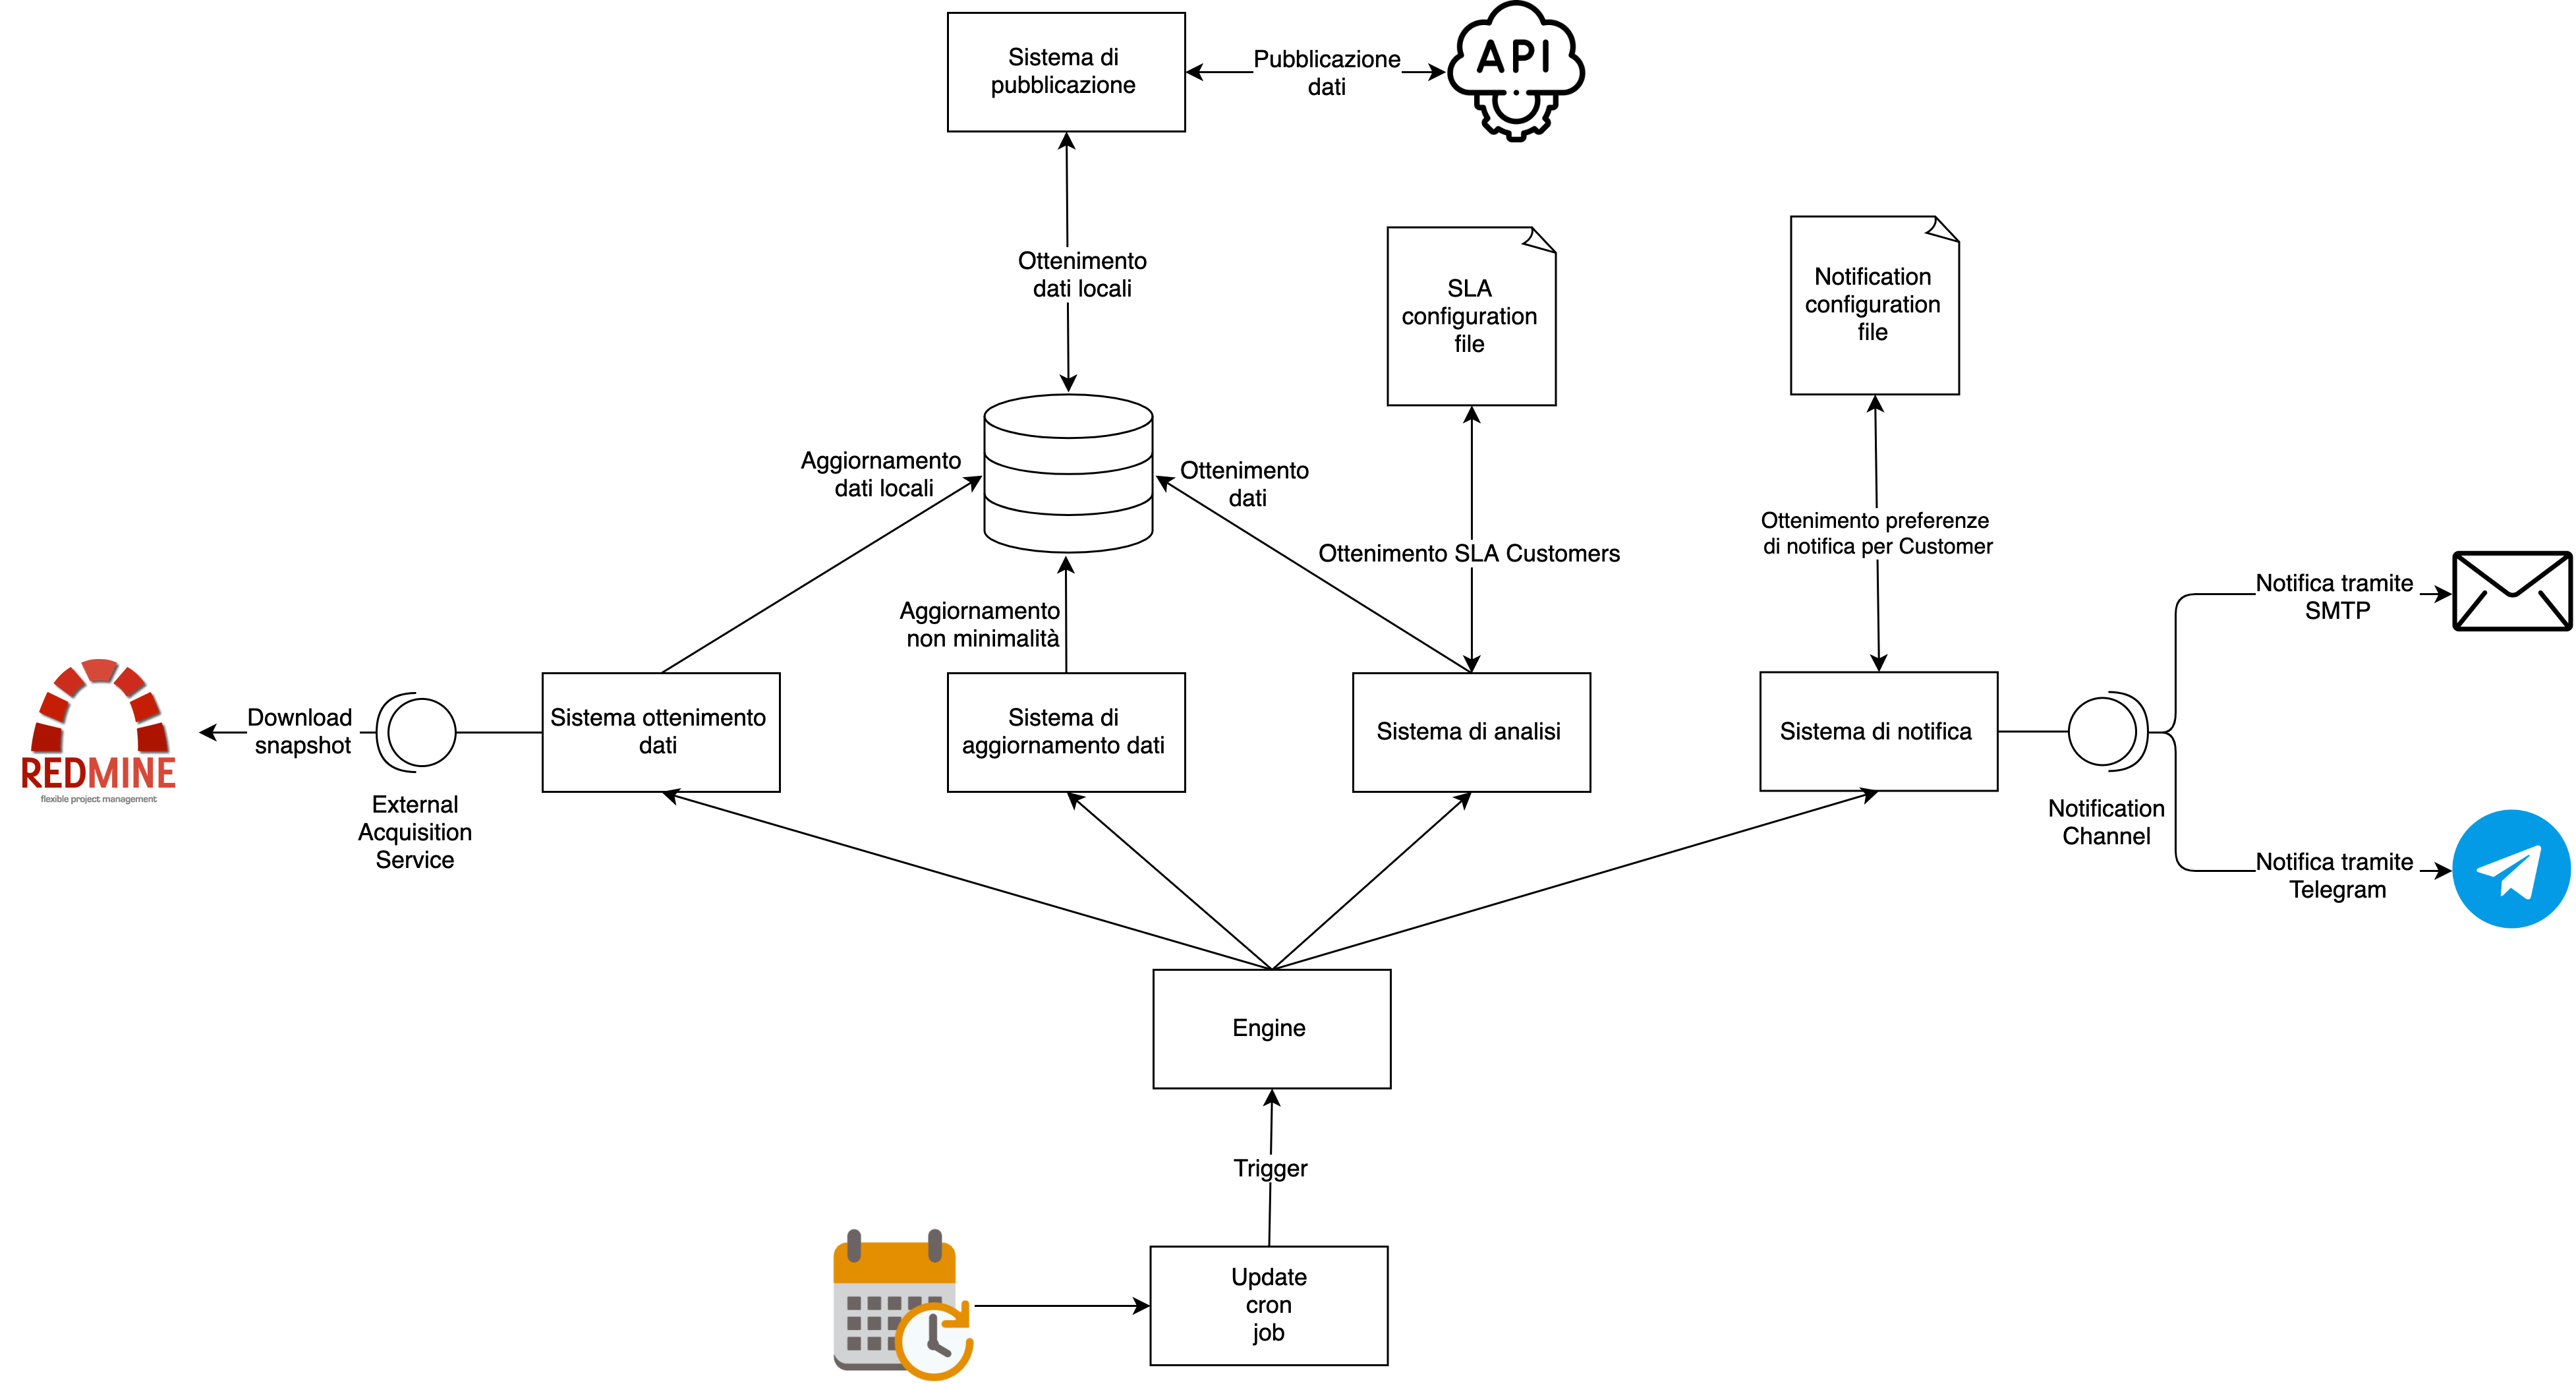
\includegraphics[keepaspectratio = true, width=16cm]{immagini/architettura-finale.png}
			\captionof{figure}{Architettura finale del progetto}
		\end{center}
		
	\subsection{Particolarità }
		Il prodotto è stato sviluppato con alcune caratteristiche ben definite fin dall'inizio come pilastri principali, quali:
		\begin{itemize}
			\item indipendenza dal provider esterno per l'ottenimento dei dati
			\item facile estensione dei canali di notifica disponibili
			\item configurabile tramite file XML
		\end{itemize}
		\subsubsection{Sistema di ottenimento}
			Il sistema di ottenimento doveva essere sviluppato tenendo a mente che un giorno si potesse migrare a un provider esterno diverso da Redmine, e che tale migrazione dovesse richiedere lo sviluppo del minor codice possibile. \\
			Tale obiettivo si è raggiunto con un esteso utilizzo di 2 design pattern, quali:
			\begin{itemize}
				\item Object Adapter
				\item Strategy
			\end{itemize}
			Tali design pattern si possono vedere applicati nel seguente UML che descrive l'effettiva implementazione di questo sistema:
   			\begin{center}
				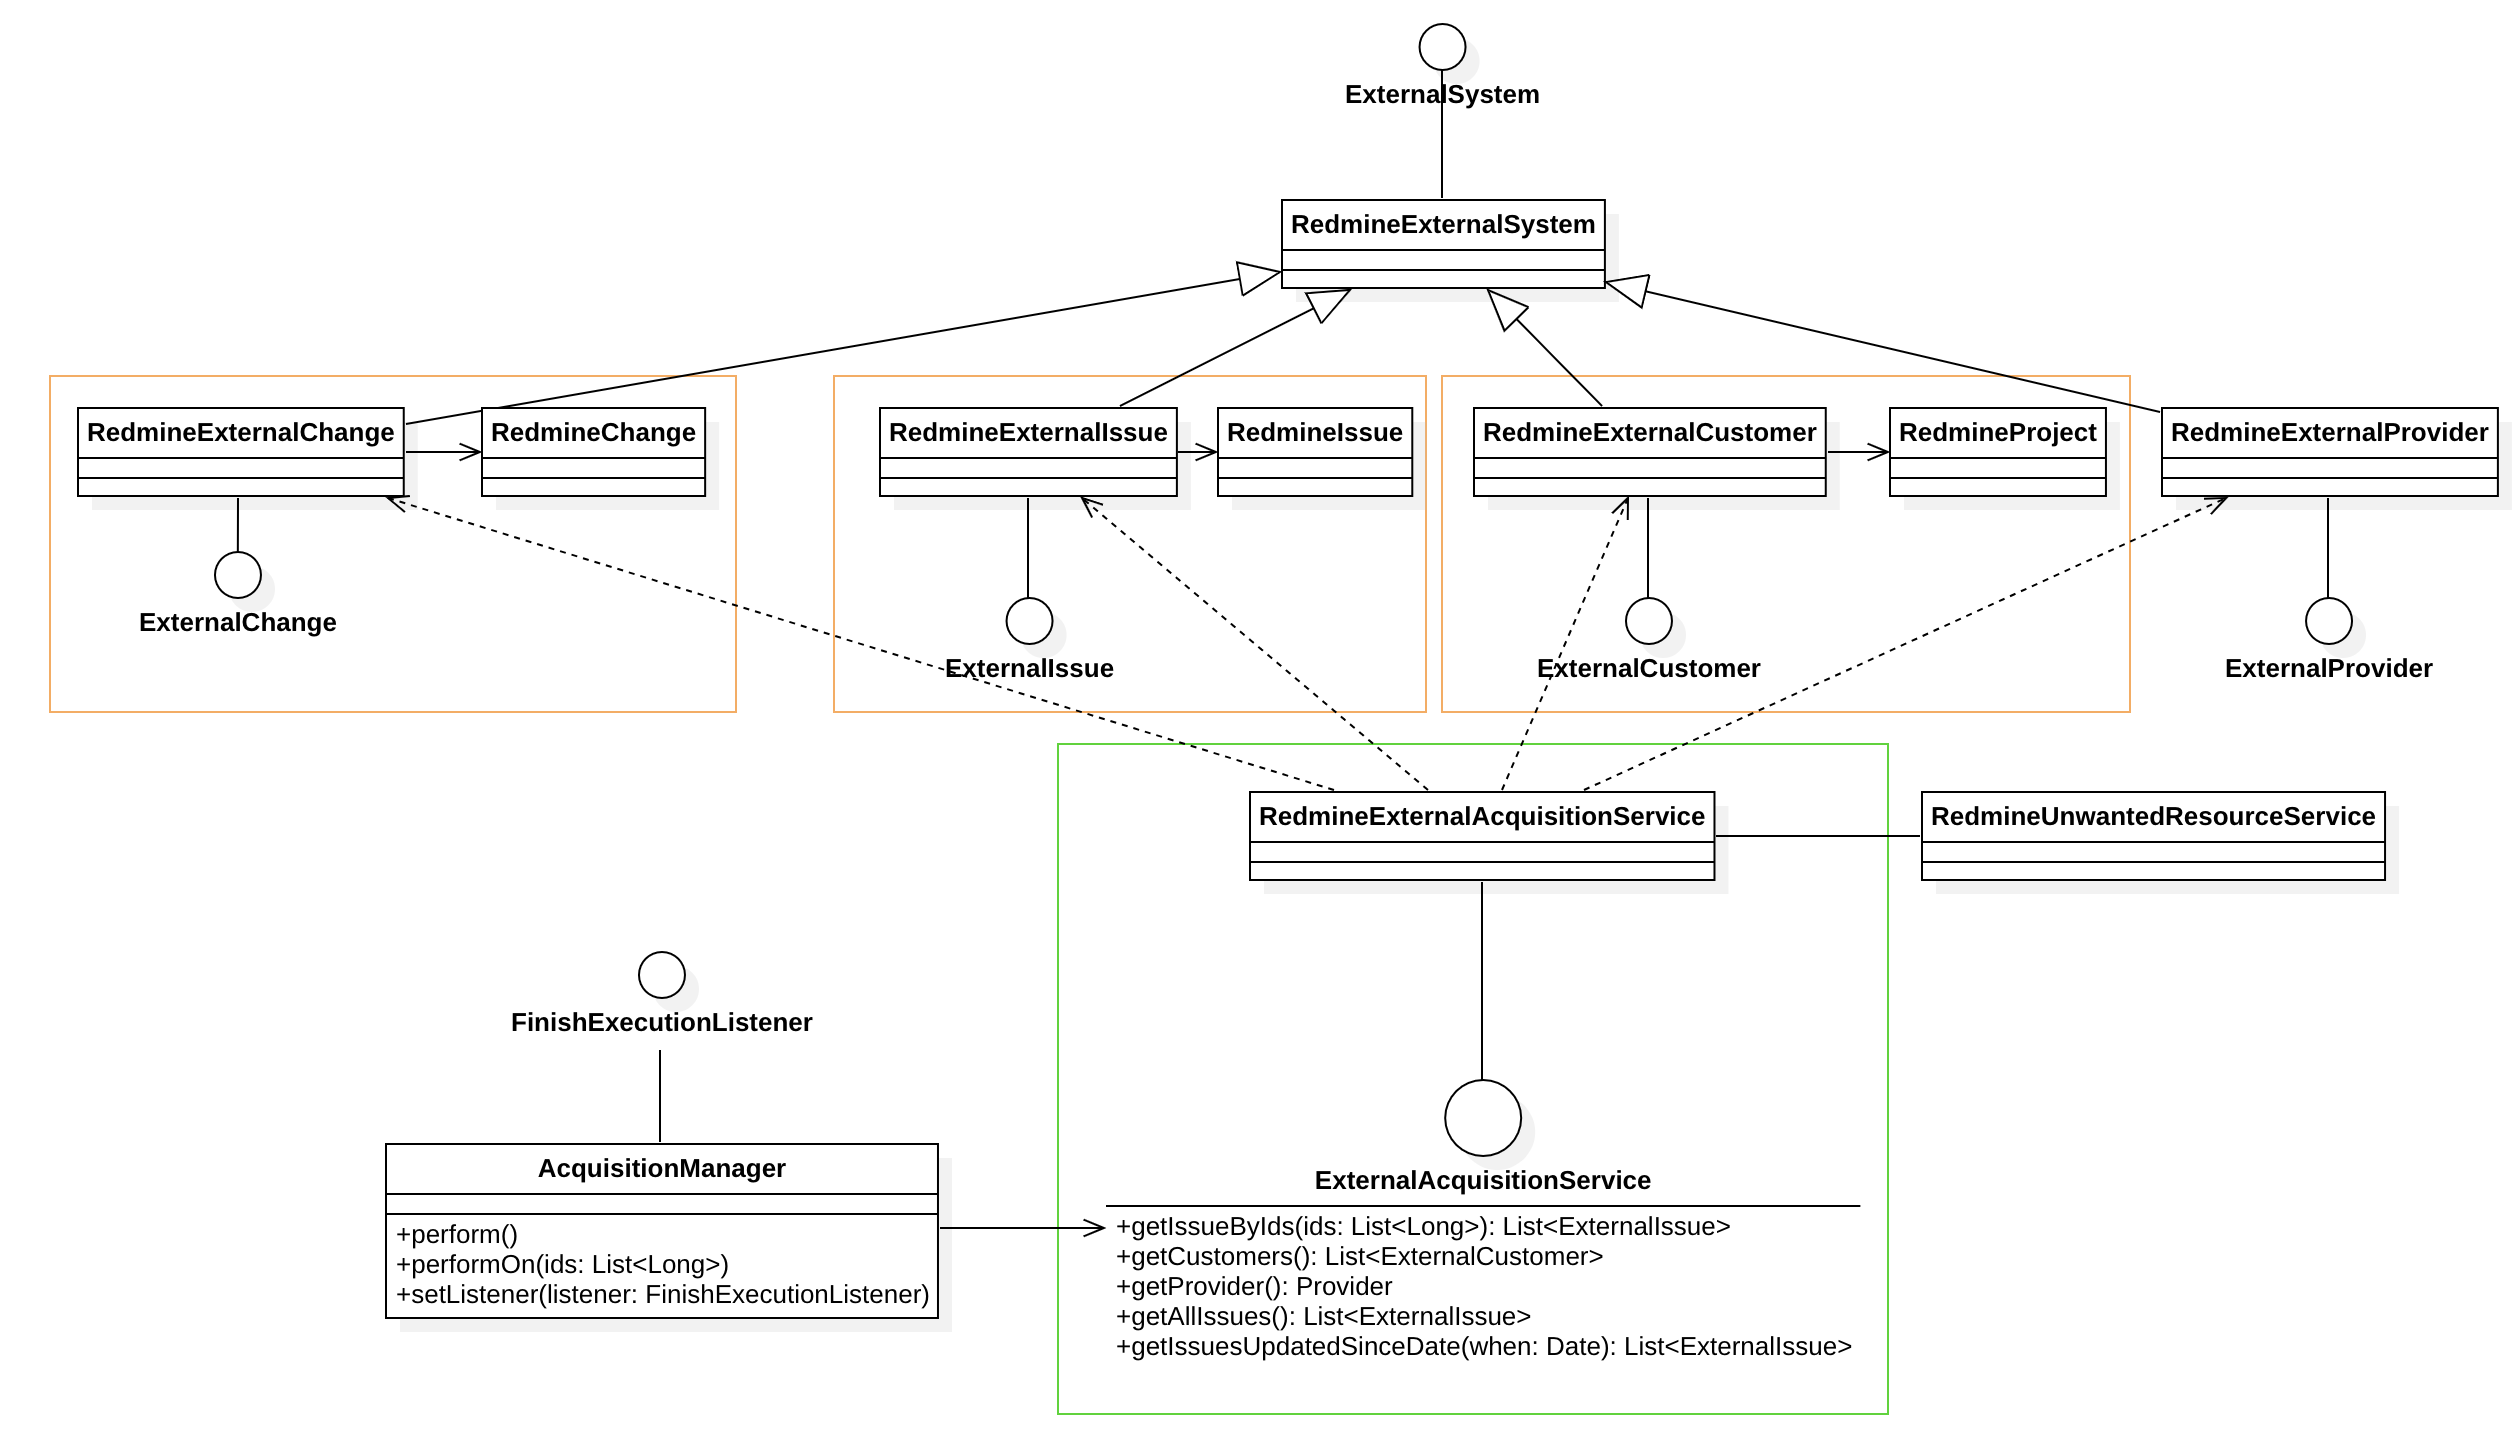
\includegraphics[keepaspectratio = true, width=16cm]{immagini/ottenimento.png}
				\captionof{figure}{UML sistema di ottenimento dati}
			\end{center}
			In arancione si denota l'applicazione del design pattern Adapter, mentre in verde l'applicazione del design pattern Strategy. \\
			Come si può notare, la classe responsabile della logica di ottenimento dei dati, \texttt{AcquisitionManager}, si interfacci al sistema esterno di ottenimento dati tramite un interfaccia, la quale definisce i metodi necessari per la strategy da implementare, e che tale strategy gestisca dati (parametri e valore di ritorno) che a loro volta sono interfacce usate per l'implementazione del design pattern Adapter: son state poi sviluppate quindi le classi adapter necessarie per adattare i vari oggetti restituiti dall'SDK di Redmine, a tali interfacce.\\
			In questo modo, se un domani si decidesse di cambiare provider, sarà necessario l'implementazione delle strategy \texttt{ExternalAcquisitionService} e dei relativi adapter per i dati ottenuti, mentre la logica di gestione di tali dati rimarrà invariata, al mantenimento degli invarianti richiesti dalle interfacce.\\
		\subsubsection{Sistema di notifica}
			Il sistema di notifica doveva essere sviluppato in modo da permettere l'implementazione di nuovi sistemi di notifica.\\
			A tale requisito, si è scoperto in fase di codifica anche la necessità di permettere politiche di invio diverse per ogni canale, in quanto per esempio, Telegram non permette l'invio di più di 20 messaggi al minuto, mentre Gmail permette l'invio di al massimo 60 mail al minuto. \\
			Per far fronte al primo requisito, si è utilizzato il design pattern Strategy per lo sviluppo dei vari canali, mentre per il secondo si è usato il meccanismo del Double Dispatch fornito dal design pattern Visitor.\\
			Tali design pattern possono essere osservati nel seguente diagramma UML, che descrive l'effettiva implementazione di questo sistema:
			\begin{center}
				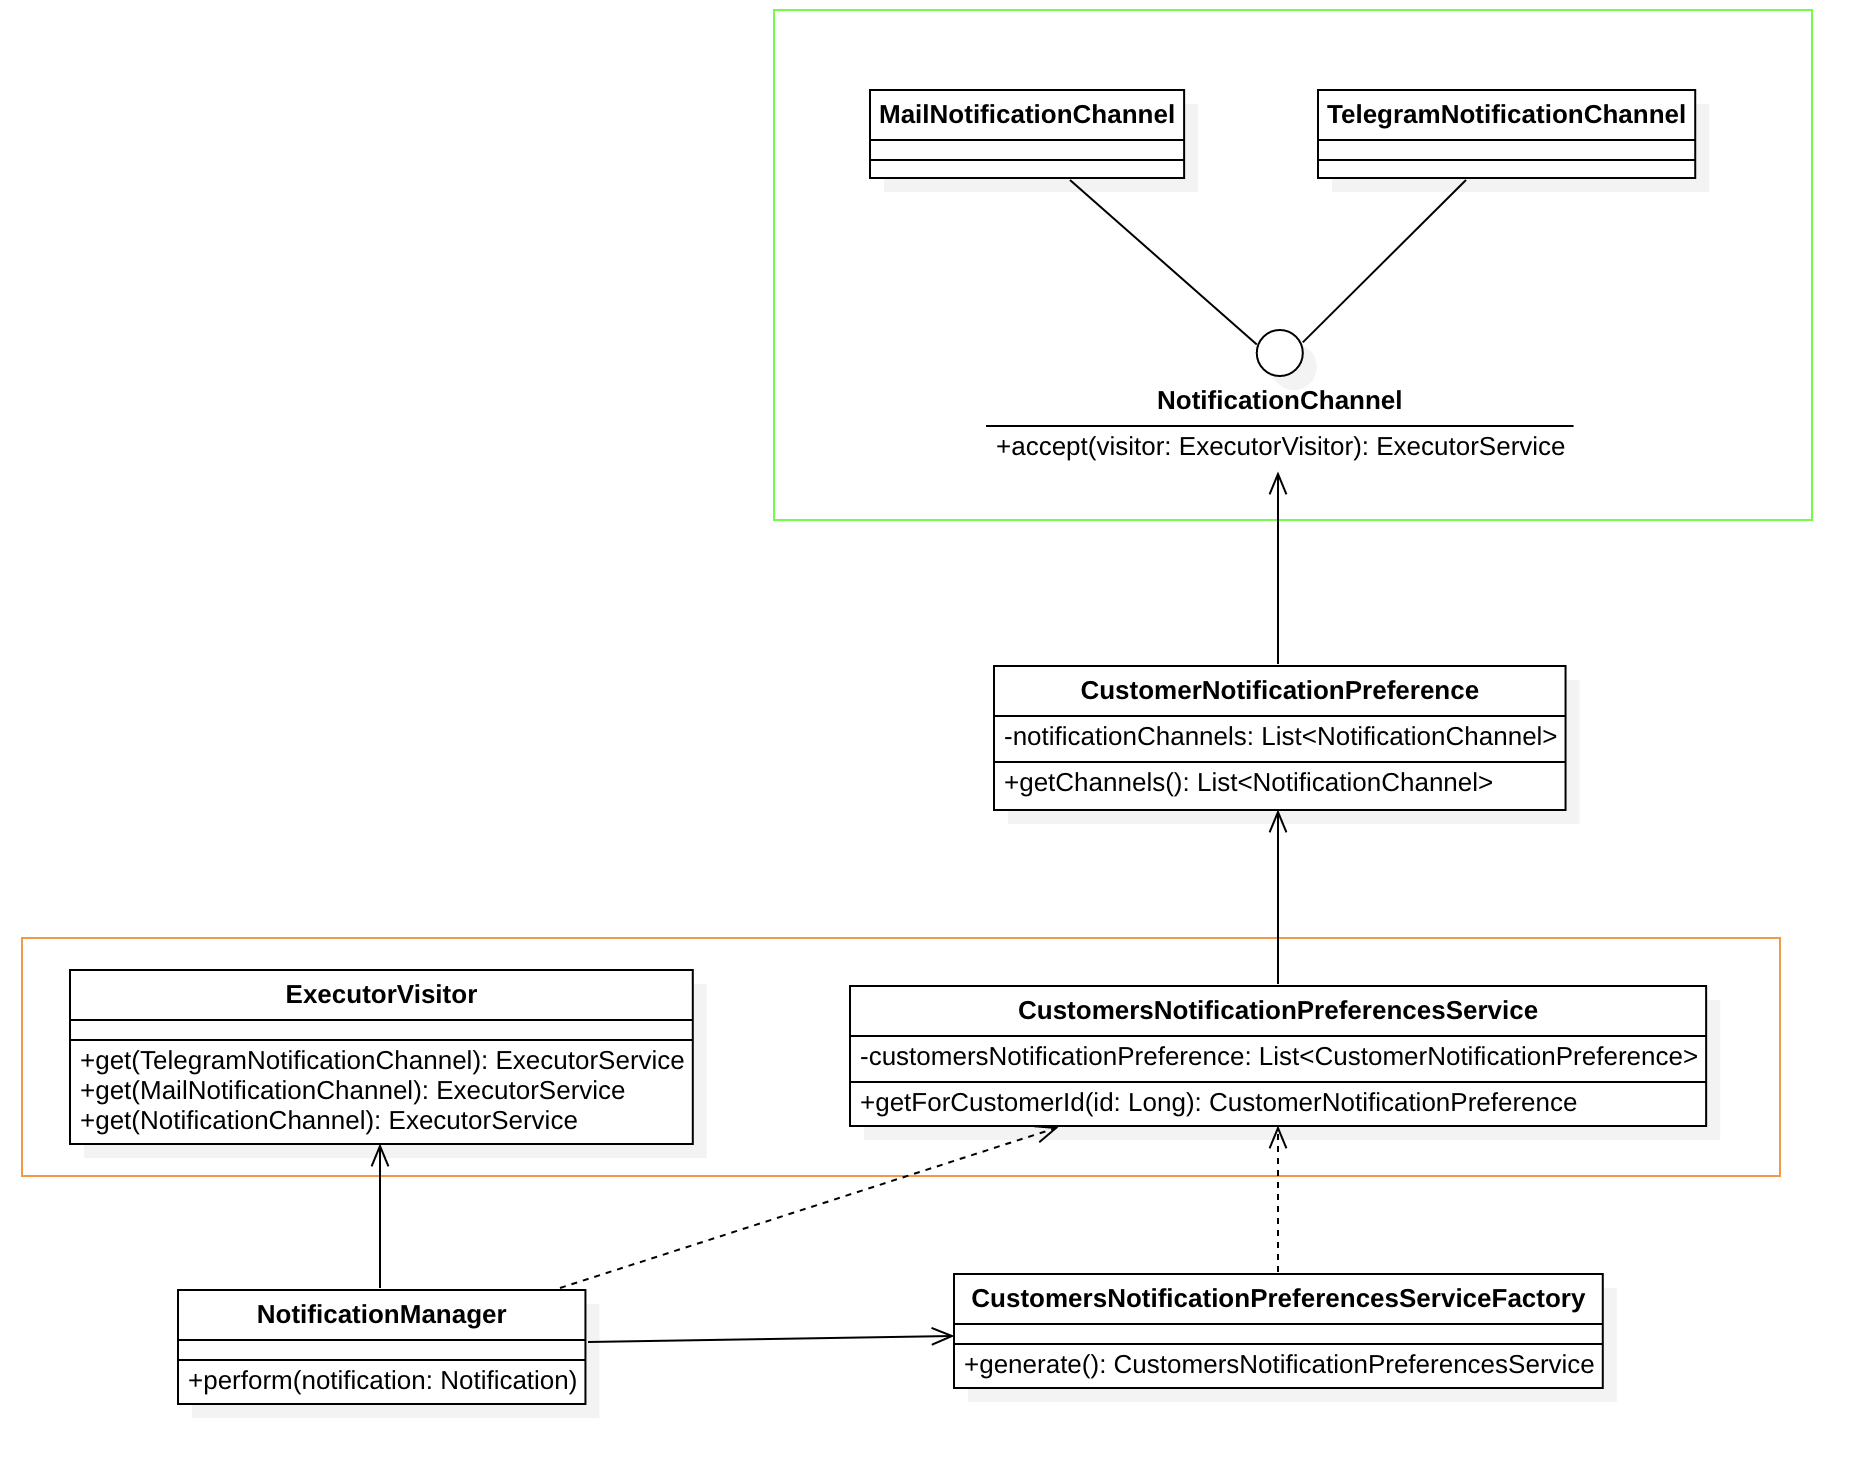
\includegraphics[keepaspectratio = true, width=16cm]{immagini/notifica.png}
				\captionof{figure}{UML sistema di notifica}
			\end{center}
			In giallo si può vedere l'applicazione del design pattern Visitor, che permetterà al sistema di ottenere un \texttt{ExecutorService} dedicato per ogni canale di notifica, e uno di default nel caso fossero presenti canali di notifica senza particolari esigenze di rate limiting. \\
			In particolare, per Telegram ritornerà un \texttt{ExecutorService} con pause di 3 secondi tra ogni \texttt{Runnable} fornitogli,  per Mail ritornerà un \texttt{ExecutorService} con pause di 0.5 secondi tra ogni \texttt{Runnable} fornitogli, mentre per il canale di default ritornerà un \texttt{CachedExecutorService} che permetterà il riutilizzo di \texttt{Thread} già istanziati.\\
			In verde invece si può vedere la strategy applicata ai due canali identificati durante la fase di analisi dei requisiti, la quale permetterà l'estensione a qualsiasi altro canale di notifica, a patto che implementi la sua interfaccia.\\
		\subsubsection{Gestione della configurazione}
			Il progetto richiedeva la possibilità di definire alcuni dati tramite file esterni. \\
			Alcune di queste informazioni sono:
			\begin{itemize}
				\item SLA dei customer (e SLA di default)
				\item orari di lavoro dei customer (e orario di default)
				\item canali di notifica per ogni customer (e canali di default)
				\item orario di lavoro dell'azienda
			\end{itemize}
			Tali file dovevano essere esterni al progetto così che, una volta creato il JAR e fatto il deploy, fosse possibile modificarli.\\
			Per ottenere ciò, son state create delle Factory per tali oggetti, che quando richiesto, andranno a deserializzare i file XML richiesti, con alcune politiche di fallback in caso di errore di lettura. \\
			All'avvio poi, basterà passare come parametro di esecuzione il path al quale sono presenti questi file.\\
		\subsubsection{Engine}
			Con \texttt{Engine}, come si può vedere nell'immagine di inizio capitolo, è l'orchestratore dei vari sistemi. \\
			Esso è responsabile dell'esecuzione dei vari manager dei sistemi nel ordine corretto, e nel caso, della gestione degli errori. \\
			Essendo i vari sistemi stati sviluppati per essere usati ad eventi, l'implementazione di questo servizio non dovrà altro che collegare i vari listeners dei manager, con i relativi eventi. \\
\iffalse			L'\texttt{Engine} sviluppato, infine, ha una logica di aggiornamento che potrebbe essere riassunta con il seguente schema:
			\begin{center}
				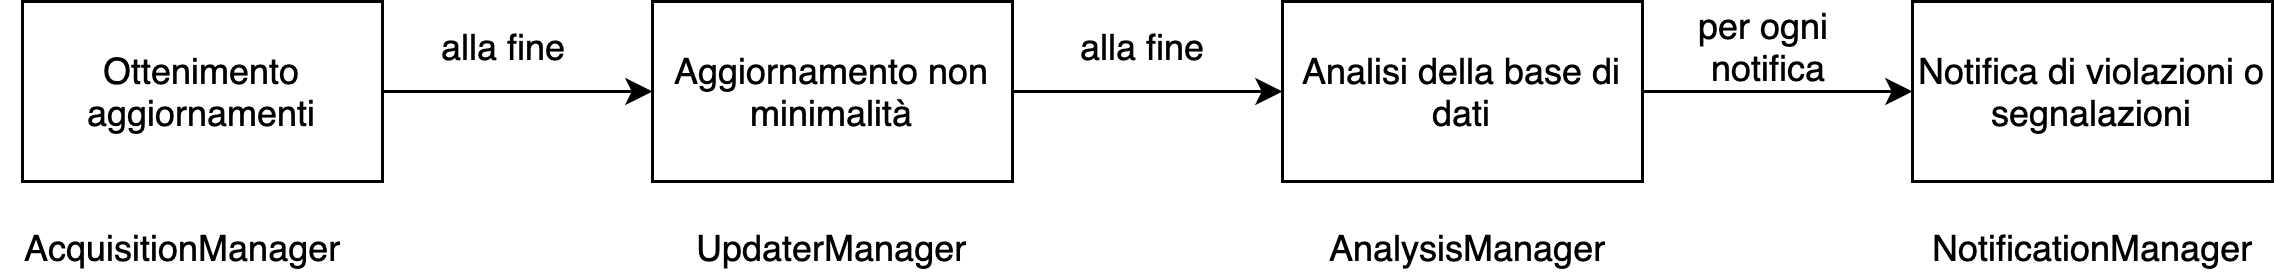
\includegraphics[keepaspectratio = true, width=16cm]{immagini/engine.png}
				\captionof{figure}{Logica di aggiornamento dell'Engine}
			\end{center} \fi
	\subsection{Extra}
		Considerato che lo sviluppo del progetto ha richiesto meno del previsto, si è proceduti allo sviluppo di feature aggiuntive esterne al progetto, quali:
		\begin{itemize}
			\item Dashboard Grafana per l'analisi dei dati presenti nella base di dati
			\item Docker container per il deploy dell'intero progetto, comprendente di engine, dashboard Grafana e database PosgreSQL
		\end{itemize}
		\subsubsection{Grafana}
			Grafana è uno progetto open-source che mira a semplificare la creazione di dashboard dinamiche per vari tipi di basi di dati. Supporta infatti basi di dati relazionali, a grafo e non relazionali.\\
			Si è proceduto quindi alla creazione di un DataSource per Grafana per la connessione al database usato, e successivamente a una Dashboard connessa a tale DataSource per la visualizzazione di alcuni highlight della base di dati. \\
			Tale dashboard è la seguente:
			\newpage
			\begin{center}
				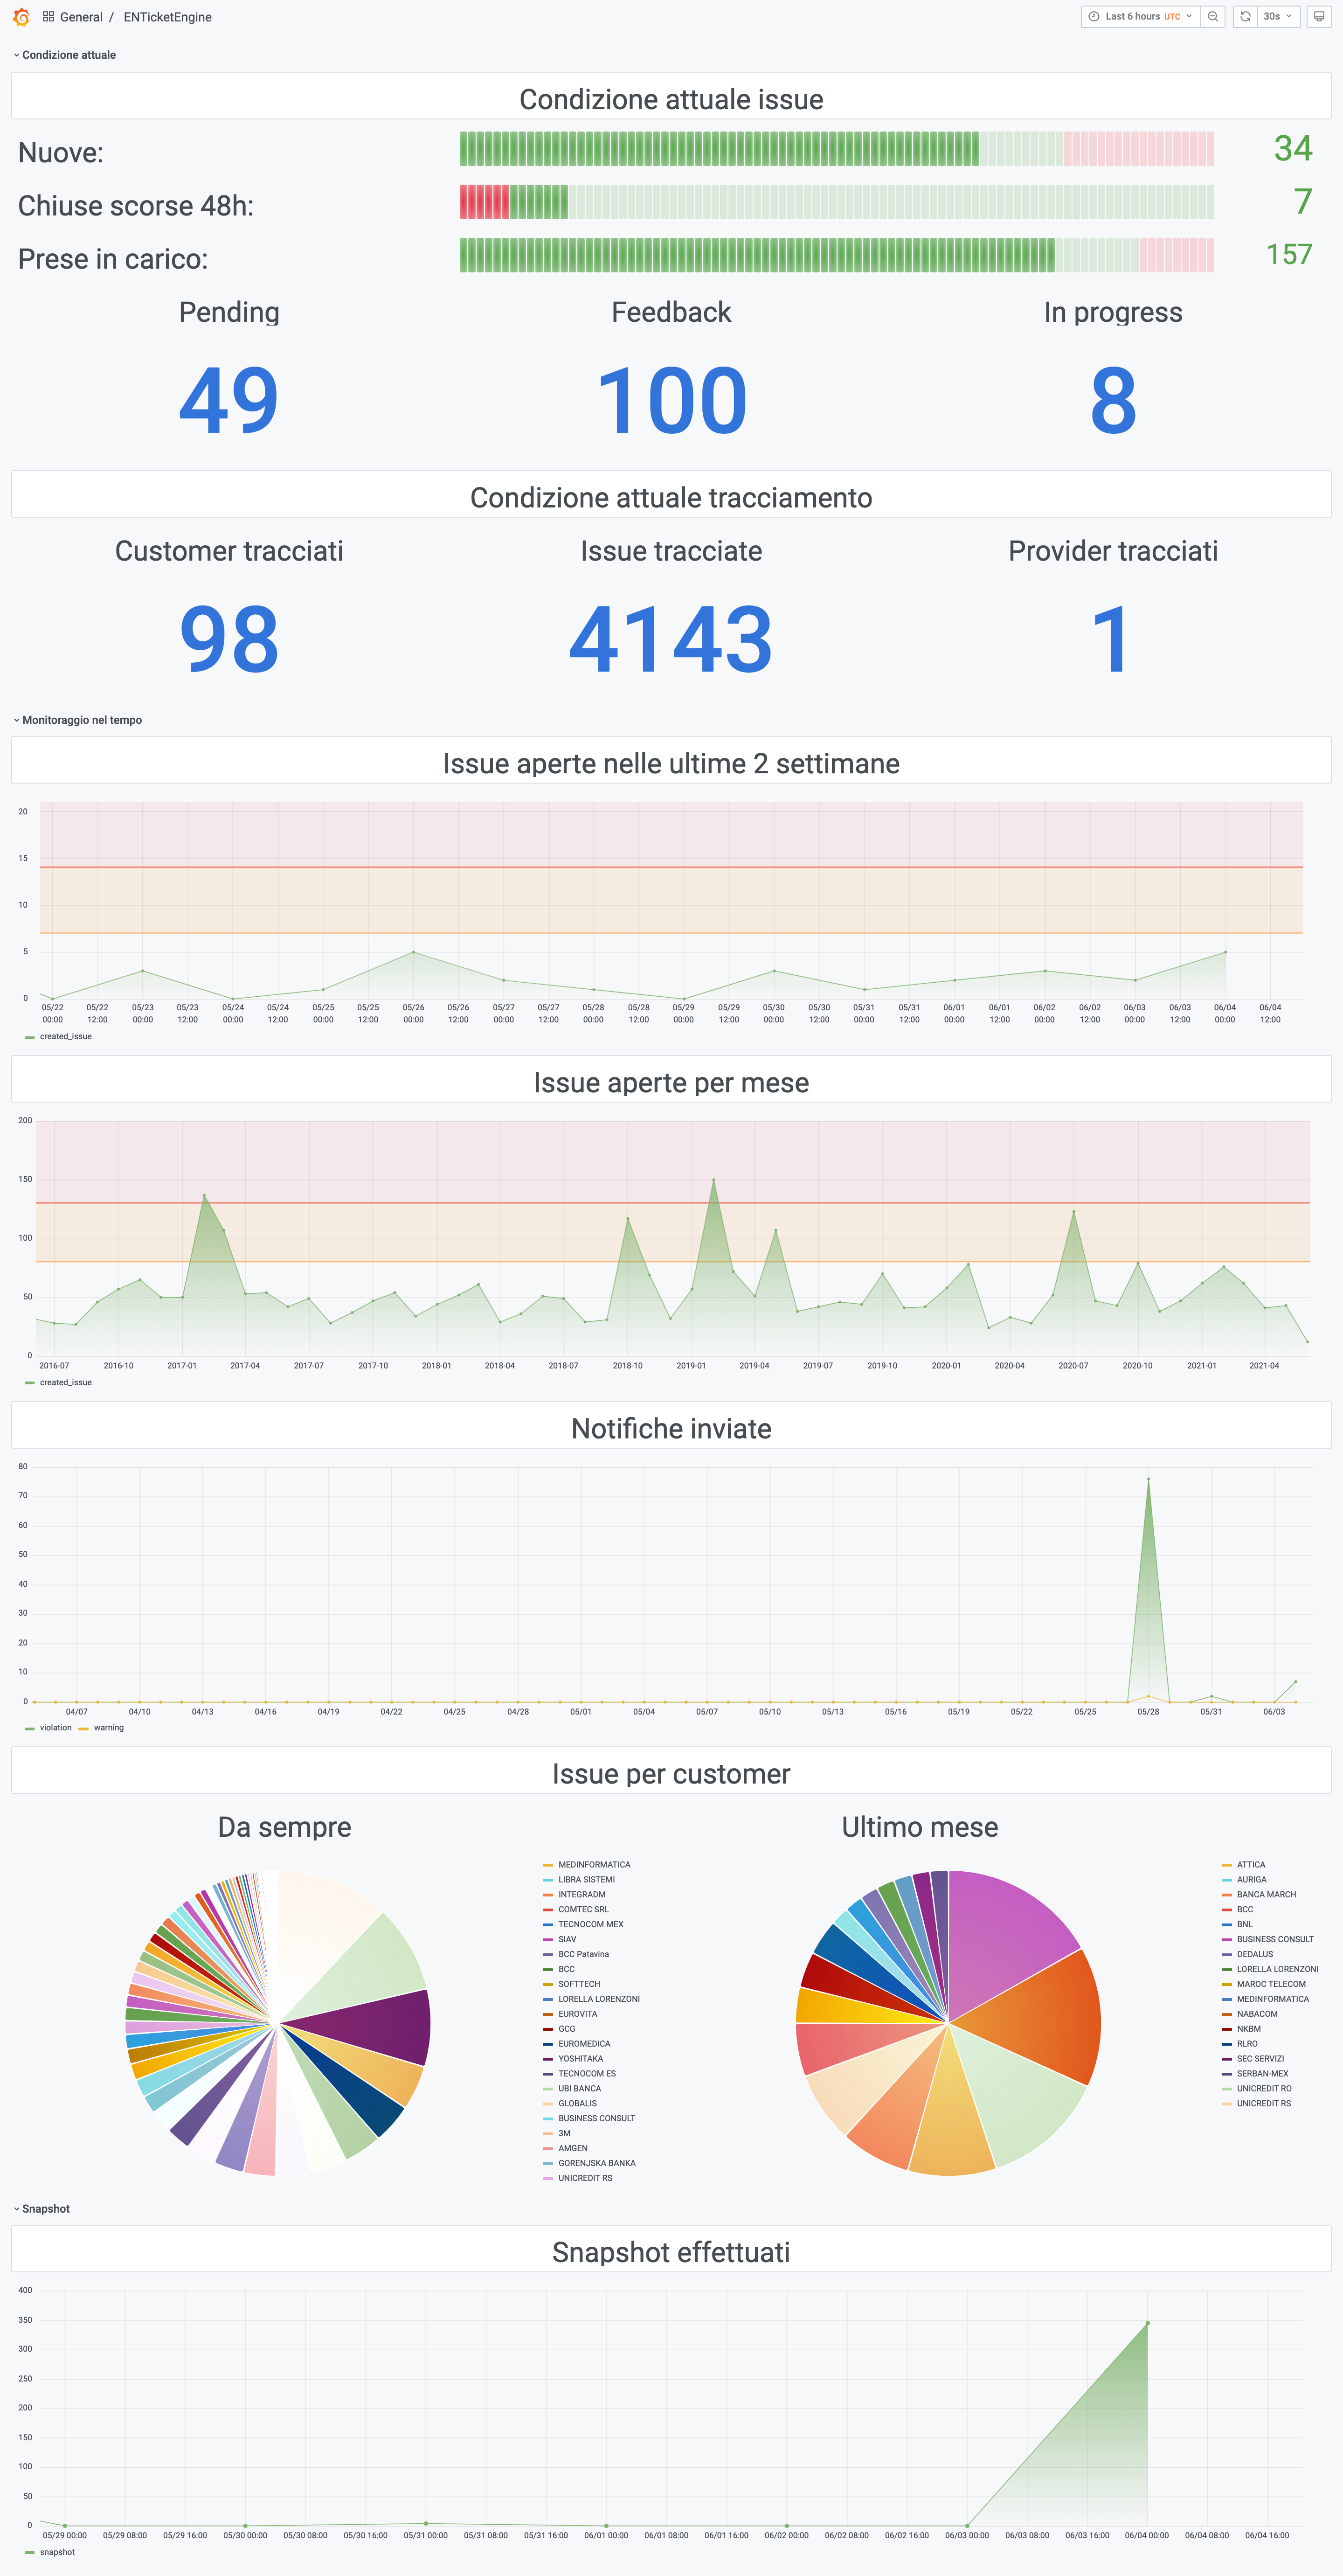
\includegraphics[keepaspectratio = true, height=20cm]{immagini/dashboard.png}
				\captionof{figure}{Dashboard Grafana}
			\end{center}
			Essa mira a mostrare un'analisi istantanea della condizione della base di dati, come il numero di ticket ancora aperti o quanti son state chiusi nelle scorse 48 ore, e un analisi nel tempo dell'andamento dei ticket.
		\subsection{Docker}
			Essendo il progetto sviluppato, completo e funzionante, si è deciso di procedere al deploy. Sfortunatamente l'azienda non disponeva di server liberi nel quale procedere all'installazione dei vari servizi necessari per il funzionamento del prodotto, quindi si è proceduto alla creazione di Dockerfile per un deploy su un DockerEngine.\\
			In particolare, si è creato un Dockerfile per l'engine, con al suo interno tutti gli step necessari per il suo deploy, e un \texttt{docker-compose.yml} per il deploy di tutte e tre le parti; in questo file erano quindi presenti 3 service quali:
			\begin{itemize}
					\item \texttt{engine }: service per il deploy del prodotto sviluppato
					\item \texttt{database }: service per il deploy della base di dati, creazione del database e popolamento di esso
					\item \texttt{granafa }:  service per il deploy di Grafana e per l'importazione della sua DataSource e Dashboard
			\end{itemize}
			Grazie a ciò, si è permesso un deploy semplice e riproducibile in qualsiasi server, tramite il comando \texttt{docker compose up}, senza la necessità di interventi sul server effettivo. Ciò ha inoltre standardizzato le cartelle all'interno del container dell'engine, permettendo un più facile configurazione dei file XML esterni.\\
			Infine, questo ha permesso una più facile definizione delle variabili di ambiente necessarie per il corretto funzionamento dei vari sistemi.
			
	\subsection{Problematiche riscontrate}
		La fase di codifica si è conclusa con l'adempimento di tutti i requisiti individuati durante la fase di analisi dei requisiti, e i requisiti successivamente individuati durante la fase stessa di codifica, come Grafana, Docker e aggiunte descritte nel paragrafo precedente.\\
		Di seguito vengono esposti le problematiche principali riscontrate durante lo sviluppo di questo progetto, e la relativa soluzione adottata:
		 \begin{center}
			\rowcolors{2}{lightest-grayest}{white}
			\begin{longtable}{|p{7cm}|p{7cm}|}
				\hline
				\rowcolor{lighter-grayer}
				\textbf{Problema} & \textbf{Soluzione} \\
				\hline
				\endfirsthead
				Bug SDK Redmine che non permetteva l'inserimento di più filtri con la medesima chiave nella stessa richiesta & Risolto: inizialmente si aveva provato a risolvere tramite la Reflection di Java, andando a cambiare il comportamento del metodo che causava ciò, ma infine si è riusciti a ottenere il comportamento ottenuto anche con la libreria standard, usando un solo parametro\\ \hline
				File XML di configurazione esterni potevano essere invalidi o assenti & Risolto: si son previsti dei file contenenti le informazioni da usare "di default" in caso quelli principali fossero malformati o assenti, e se anch'essi avessero problemi, degli oggetti di default hardcoded nel programma, così da avere sempre uno stato funzionante dell'engine\\ \hline
				Lo storico delle issue non doveva sollevare notifiche & Risolto: si è previsto una logica di analisi che permette di evitare di inviare notifiche di segnalazione o violazione in caso quel ticket fosse stato già segnalato \\ \hline
				L'applicativo ha dipendenze sul sistema non triviali per il deploy & Risolto: inizialmente si aveva provato a creare uno script di installazione, che procedesse a installare tutti i sistemi necessari per l'esecuzione, ma infine si è optato per l'uso di Docker in quanto prodotto standard usato esattamente per questo obbiettivo \\ \hline
			\end{longtable}
		\end{center}